% Provenance (never printed): see sources/outline_sources.md (Year 3: the
% structure of the Galaxy; the rotation curve and dark matter; galaxy types;
% the distance ladder, Hubble's law recalled from the physics books).
% Brief: sources/book5/BRIEFS.md, ch. 29. Curves from figdata/bachelor-3/
% rotation_curve.py (the circular velocity curve of Eilers et al. 2019 with the
% Pouliasis et al. 2017 Model I baryons and an NFW halo fitted to it) and
% distance_ladder.py (the OGLE-IV Cepheids of the Large Magellanic Cloud, CDS
% J/AcA/65/297, and the ranges of the rungs). Exercise and problem values in the
% Book 5 scratch calculator calc/ch29.py. The survey of Part I of the problem and
% the galaxies of the exercises are invented.
\chapter{Bima Sakti dan Galaksi-Galaksi}\label{ch:b3:milky-way-galaxies}

Di Tata Surya, planet-planet yang jauh dari Matahari bergerak lambat: Merkurius
mengelilinginya dengan kecepatan \qty{47.4}{km.s^{-1}}, Neptunus dengan \qty{5.4}{km.s^{-1}}, sebagaimana
hukum ketiga Kepler mensyaratkannya untuk benda-benda yang terikat pada satu massa pusat. Bintang-bintang
di Galaksi tidak berperilaku demikian. Diukur dari gerak lebih dari
dua puluh ribu raksasa merah, kelajuan orbit melingkar mereka adalah
\qty{227}{km.s^{-1}} pada jarak \qty{5}{kpc} dari pusat, \qty{229}{km.s^{-1}}
di Matahari, dan masih \qty{198}{km.s^{-1}} pada \qty{25}{kpc}, tempat hampir
tidak ada lagi bintang atau gas. Jika massa yang kita lihat adalah seluruh massa yang ada, bintang-bintang
di pinggiran akan jauh lebih lambat. Ada sesuatu yang tak terlihat yang menahan mereka. Bab ini
menguraikan Galaksi tempat kita tinggal, menimbangnya dari rotasinya, mengelompokkan
galaksi-galaksi lain ke dalam tipe-tipenya, dan menelusuri rangkaian metode
yang dipakai untuk mengukur jarak mereka serta pengembangan Alam Semesta.
% ledger: planet:Mercury.vorb, planet:Neptune.vorb, eilers19:vc, eilers19:table1

\begin{recall}
Bima Sakti, efek Doppler, hukum Kepler, teorema Newton tentang
tarikan kulit bola, materi gelap, lubang hitam dan
jari-jari Schwarzschild, supernova, katai putih, garis 21-cm dari
hidrogen atom, dan hukum Hubble dibahas dalam buku fisika. Paralaks tahunan,
parsek, fluks dan luminositas, magnitudo semu dan mutlak, serta
modulus jarak, pita fotometrik, dan indeks warna dibahas dalam
volume Tahun~1, pada bab tentang teleskop dan fotometri. Medium
antarbintang dan debunya dibahas dalam volume Tahun~2, pada bab tentang
medium antarbintang dan pembentukan bintang.
\end{recall}

\section{Struktur Galaksi}\label{sec:b3:milky-way-galaxies:structure}

Dilihat dari Bumi, Galaksi tampak sebagai Bima Sakti: pita cahaya yang melingkari
seluruh langit, dilintasi jalur-jalur debu gelap dan paling terang ke arah
rasi Sagittarius, tempat pusatnya berada. Pita ini adalah cakram tempat
Matahari berada, yang terlihat dari dalam dengan sudut pandang tepi.

\begin{omfigure}
\centering
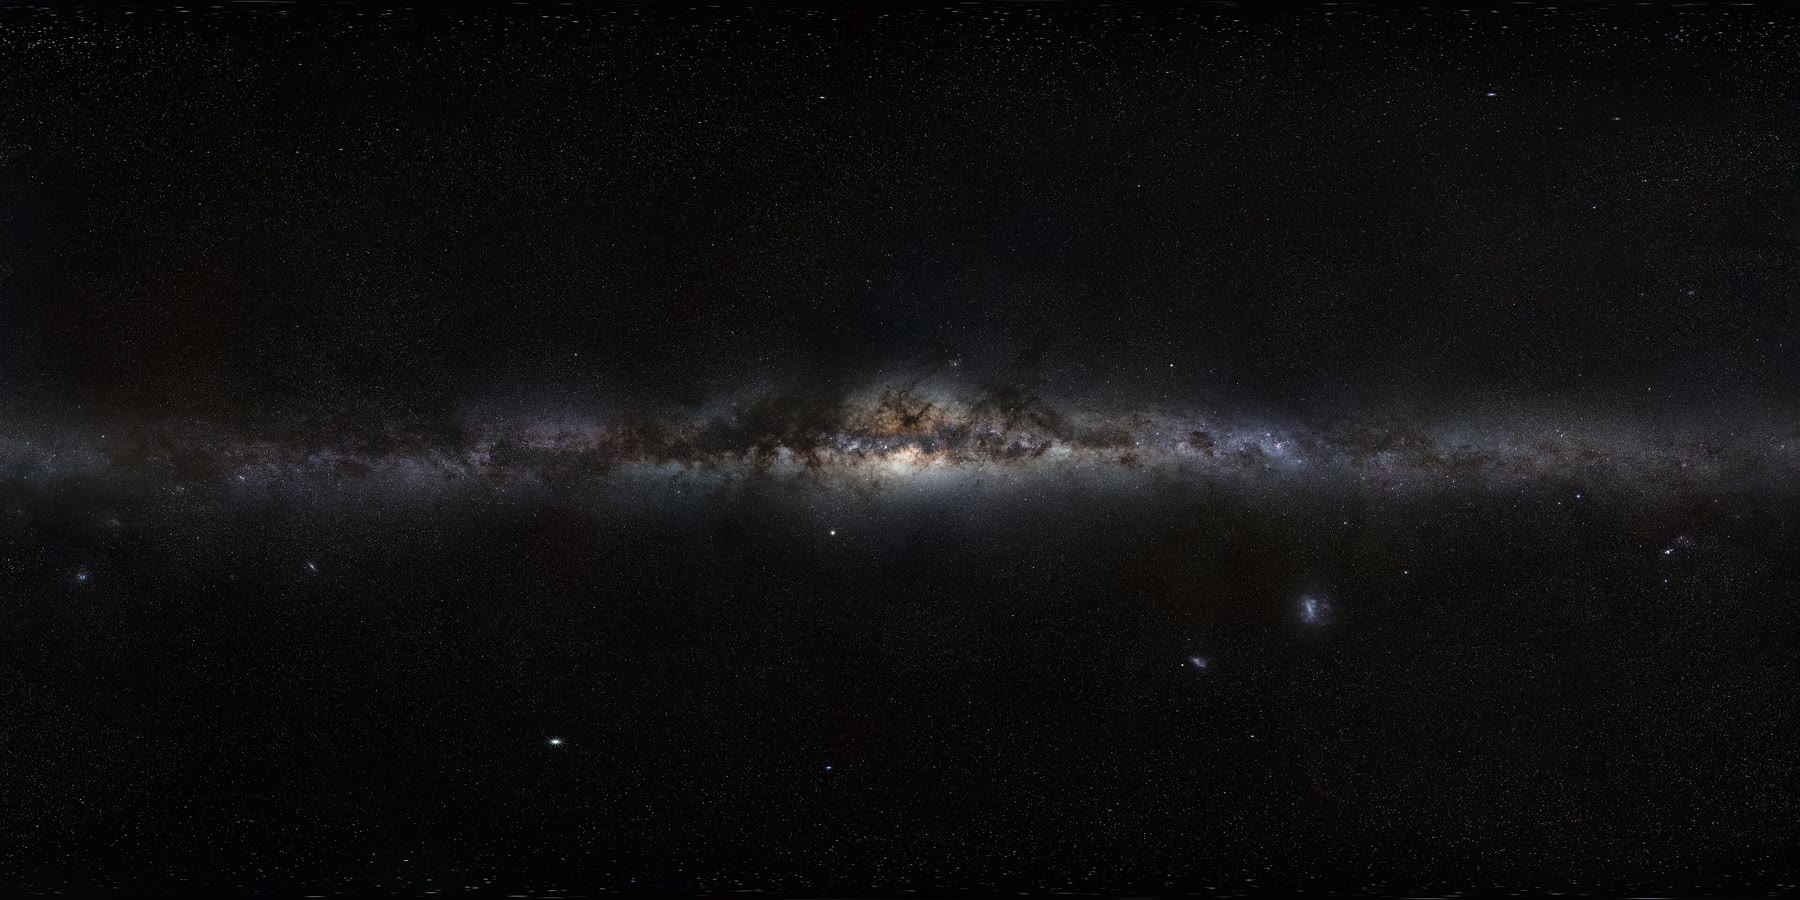
\includegraphics[width=0.96\linewidth]{images/book5/b3-milky-way-panorama.jpg}
\par\smallskip{\small Seluruh langit dalam satu citra, diproyeksikan sedemikian rupa sehingga
bidang Galaksi melintang di tengah dan pusatnya berada di
tengah gambar. Pita ini adalah cakram yang terlihat dari dalam; jalur-jalur gelap
adalah debu di dalam cakram yang menutupi bintang di belakangnya; tonjolan pusat
membengkak di sekitar pusatnya. Dua bercak kecil di bawah pita, di sebelah
kanan, adalah Awan Magellan Besar dan Awan Magellan Kecil, dua galaksi satelit;
bercak samar di bawah pita dekat tepi kiri adalah
galaksi Andromeda. Foto ESO/S.~Brunier, CC BY~4.0.}\label{fig:b3:milky-way-galaxies:panorama}
\end{omfigure}
% ledger: photo:b3-milky-way-panorama, mcconn12:local-group

\begin{definition}[Cakram Galaksi, cakram tebal, tonjolan Galaksi, dan halo bintang]\label{def:b3:milky-way-galaxies:structure}
Yang disebut \emph{cakram Galaksi}\index{cakram Galaksi} adalah komponen Galaksi yang pipih, terdiri atas
bintang, gas, dan debu yang bergerak dalam orbit hampir melingkar mengelilingi pusatnya;
kerapatannya turun kira-kira secara eksponensial terhadap tinggi di atas
bidang tengahnya dan terhadap jarak dari pusatnya, dengan skala tinggi dan skala
panjang. \emph{Cakram tebal}\index{cakram tebal} adalah komponen cakram kedua yang lebih tua,
dengan skala tinggi yang lebih besar dan massa yang lebih kecil. Yang disebut
\emph{tonjolan Galaksi}\index{tonjolan Galaksi} adalah konsentrasi bintang di bagian tengah
yang membengkak keluar dari cakram. Adapun \emph{halo bintang}\index{halo bintang}
adalah komponen yang jarang dan kira-kira berbentuk sferoid, berisi bintang-bintang tua dan
gugus bola yang mengelilingi cakram dan tonjolan.
\end{definition}

Bima Sakti adalah \omterm{def:b3:milky-way-galaxies:types}{galaksi spiral} berpalang. Di sekitar Matahari, cakram tipis
memiliki skala tinggi sekitar \qty{300}{pc} dan \omterm{def:b3:milky-way-galaxies:structure}{cakram tebal}
sekitar \qty{900}{pc}; skala panjang keduanya sekitar \qty{2.6}{kpc} dan
\qty{2.0}{kpc}. \omterm{def:b3:milky-way-galaxies:structure}{Cakram tebal} memuat sekitar \num{6e9} massa Matahari,
kira-kira seperlima cakram tipis. Dilihat dari samping, tonjolan berbentuk kotak
atau kacang: ia adalah bagian dalam palang bintang yang menebal, dengan
panjang setengah sumbu sekitar \qty{5}{kpc}, yang sumbu panjangnya membentuk
sudut \ang{27} terhadap garis dari Matahari ke pusat. \omterm{def:b3:milky-way-galaxies:structure}{Halo bintang} hanya memuat
sekitar satu persen bintang. Secara keseluruhan, bintang-bintang di Galaksi
memiliki massa sekitar \num{5e10} massa Matahari.
% ledger: bhg16:structure

\begin{omfigure}
\centering
\begin{tikzpicture}[x=0.17cm, y=0.17cm, font=\scriptsize]
% edge-on view
\begin{scope}
\fill[omProp!8] (0,0) circle (17);
\draw[omProp!60, densely dotted] (0,0) circle (17);
\fill[black!12] (0,0) ellipse (15 and 2.4);
\fill[black!30] (0,0) ellipse (15 and 0.8);
\fill[black!45] (-3.2,0) .. controls (-3.4,2.3) and (-1.2,2.0) .. (0,1.4)
  .. controls (1.2,2.0) and (3.4,2.3) .. (3.2,0)
  .. controls (3.4,-2.3) and (1.2,-2.0) .. (0,-1.4)
  .. controls (-1.2,-2.0) and (-3.4,-2.3) .. (-3.2,0) -- cycle;
\foreach \p in {(-10,9),(6,12),(12,-7),(-6,-13),(-13,-4),(3,-9),(12,8)}
  \fill[omProp] \p circle (0.35);
\fill[ocYellow, draw=black] (-8.2,0.15) circle (0.55);
\node[anchor=south] at (-8.2,0.9) {Matahari};
\draw[|<->|] (0,-4.6) -- node[below] {$R_0 \approx \qty{8.2}{kpc}$} (-8.2,-4.6);
\node[anchor=west] at (15.3,0) {cakram tipis};
\node[anchor=west] at (13.2,2.8) {cakram tebal};
\draw[->] (4.6,4.6) node[anchor=south west, inner sep=1pt] {tonjolan} -- (2.4,1.7);
\node[omProp!80!black] at (-11,13.5) {halo bintang};
\node at (0,-19.5) {(a) dilihat dari samping};
\end{scope}
% face-on view
\begin{scope}[xshift=7.6cm]
\fill[omProp!8] (0,0) circle (17);
\draw[omProp!60, densely dotted] (0,0) circle (17);
\fill[black!12] (0,0) circle (15);
\foreach \a in {0,180} {
  \draw[line width=1.6pt, black!40, rotate=\a+63]
    plot[domain=0:3.9, samples=50] ({5*exp(0.25*\x)*cos(\x r)}, {5*exp(0.25*\x)*sin(\x r)});
}
\fill[black!45, rotate=63] (0,0) ellipse (5 and 1.5);
\draw[dashed] (0,0) circle (8.2);
\fill[ocYellow, draw=black] (0,-8.2) circle (0.55);
\node[anchor=north] at (0,-8.9) {Matahari};
\draw[dotted, thick] (0,0) -- (0,-8.2);
\draw[thick, ->] (0,0) ++(25:16) arc (25:-25:16);
\node[anchor=west] at (17.3,0) {rotasi};
\node[anchor=west, fill=black!12, inner sep=1pt] at (3.4,3.4) {palang};
\draw[|-|] (6,-15.5) -- node[below] {\qty{5}{kpc}} (11,-15.5);
\node at (0,-19.5) {(b) dilihat dari kutub Galaksi utara};
\end{scope}
\end{tikzpicture}
\par\smallskip{\small Sketsa Galaksi, sesuai skala untuk dimensi
utamanya. (a)~Dilihat dari samping: cakram tipis (pita gelap), \omterm{def:b3:milky-way-galaxies:structure}{cakram tebal} (pita
terang), tonjolan berbentuk kotak, dan \omterm{def:b3:milky-way-galaxies:structure}{halo bintang} dengan gugus bolanya
(titik oranye); Matahari berada di cakram, sekitar \qty{8.2}{kpc}
dari pusat dan sekitar \qty{25}{pc} di atas bidang tengah (terlalu kecil untuk
ditampilkan). (b)~Dilihat dari kutub Galaksi utara: palang yang
panjang setengah sumbunya sekitar \qty{5}{kpc}, miring \ang{27} terhadap garis dari
Matahari ke pusat (titik-titik); lingkaran Matahari (putus-putus); lengan spiral
digambar secara skematis; Galaksi berputar searah jarum jam dalam tampilan ini.}\label{fig:b3:milky-way-galaxies:sketch}
\end{omfigure}
% ledger: bhg16:structure, gravity19:r0

\begin{definition}[Populasi bintang]\label{def:b3:milky-way-galaxies:populations}
Yang disebut \emph{populasi bintang}\index{populasi bintang} adalah sekelompok bintang
dalam suatu galaksi yang memiliki rentang umur, komposisi kimia, dan
orbit yang serupa. Bintang-bintang muda di cakram tipis, kaya unsur yang lebih berat daripada
helium, dan berada pada orbit hampir melingkar, secara tradisional disebut
populasi~I; bintang-bintang tua di halo dan di gugus bola, miskin
unsur berat dan bergerak pada orbit dengan gerak acak yang besar serta sedikit
rotasi bersih, disebut populasi~II.
\end{definition}

\omterm{def:b3:milky-way-galaxies:structure}{Cakram tebal} berada di antara keduanya: bintang-bintangnya umumnya lebih tua daripada
bintang-bintang cakram tipis dan, pada kadar besi yang sama, lebih kaya unsur ringan
yang oleh para astronom disebut unsur alfa, diukur relatif terhadap besi. \omterm{def:b3:milky-way-galaxies:structure}{Halo
bintang} merupakan
catatan fosil. Sebagian besar halo dibentuk dari galaksi-galaksi kecil yang jatuh
ke dalam Galaksi dan tercabik oleh pasang surutnya, dan sebagian aliran
bintang dari galaksi-galaksi itu masih dapat ditelusuri di seluruh langit.
% ledger: bhg16:populations

\begin{definition}[Koordinat Galaksi]\label{def:b3:milky-way-galaxies:coordinates}
Yang disebut \emph{koordinat Galaksi}\index{koordinat Galaksi} suatu arah adalah
\emph{lintang Galaksi} $b$, yaitu sudut arah itu dari bidang Galaksi
(positif ke arah kutub Galaksi utara), dan \emph{bujur
Galaksi} $\ell$, diukur pada bidang dari arah
pusat Galaksi ($\ell = 0$) melalui $\ell = \ang{90}$, yaitu arah
ke arah mana rotasi Galaksi membawa Matahari. Bidang itu
ditetapkan pada 1958 sebagai bidang utama hidrogen atomik Galaksi;
kutub Galaksi utara terletak pada asensio rekta \ang{192.25}
($12^\mathrm{h}49^\mathrm{m}$) dan deklinasi \ang{27.4} (ekuinoks
1950).
\end{definition}
% ledger: liu11:galactic, reid20:sgra

Matahari tidak tepat berada di bidang itu: ia terletak sekitar \qty{25}{pc} di utara bidang tersebut.
Jaraknya dari pusat, $R_0$, lama menjadi besaran yang paling tidak pasti dalam
astronomi Galaksi. Kini besaran itu diukur secara geometris: bintang S2 mengelilingi
lubang hitam pusat Galaksi dalam orbit berperiode \num{16} tahun, yang
ukuran sudut di langit dan kecepatannya sepanjang garis pandang, yang diamati
selama 27 tahun, memberikan jarak ke pusat secara langsung:
$R_0 = \qty{8178}{pc}$, dengan ketidakpastian statistik \qty{13}{pc} dan
ketidakpastian sistematik \qty{22}{pc}. Tinjauan atas semua metode memberikan
$R_0 = \qty[separate-uncertainty=true]{8.2 \pm 0.1}{kpc}$.
% ledger: bhg16:structure, gravity19:r0

\section{Rotasi dan halo materi gelap}\label{sec:b3:milky-way-galaxies:rotation}

\begin{definition}[Standar diam lokal]\label{def:b3:milky-way-galaxies:lsr}
Yang disebut \emph{standar diam lokal}\index{standar diam lokal} (LSR) adalah
kerangka acuan yang bergerak pada orbit melingkar terhadap pusat Galaksi
yang melewati posisi Matahari saat ini. Kecepatan bintang dan gas di dekatnya
dinyatakan relatif terhadapnya.
\end{definition}

Matahari bergerak relatif terhadap LSR sekitar \qty{10}{km.s^{-1}} menuju
pusat Galaksi, \qty{11}{km.s^{-1}} searah rotasi, dan
\qty{7}{km.s^{-1}} menuju kutub Galaksi utara: gerak khas yang kecil
di atas orbit dengan laju $V_0$ beberapa ratus kilometer
per detik. Dilihat dari Bumi, sumber radio di pusat
Galaksi bergeser sepanjang bidang Galaksi sebesar \qty{6.411}{mas} per tahun; hampir seluruh
pergeseran itu merupakan refleksi dari orbit Matahari, dan dari situ diperoleh
kecepatan total Matahari terhadap pusat, \qty[separate-uncertainty=true]{248 \pm 3}{km.s^{-1}}
(\cref{exo:b3:milky-way-galaxies:2}).
% ledger: bhg16:lsr, reid20:sgra

\begin{definition}[Kurva rotasi; konstanta Oort]\label{def:b3:milky-way-galaxies:rotation-curve}
Yang disebut \emph{kurva rotasi}\index{kurva rotasi} suatu galaksi cakram adalah
laju $V(R)$ orbit melingkar dalam bidangnya sebagai fungsi
jarak $R$ dari pusatnya. Untuk Galaksi, dengan $V_0 = V(R_0)$ dan
$V'_0 = \mathrm{d}V/\mathrm{d}R$ pada $R_0$, \emph{konstanta
Oort}\index{konstanta Oort} adalah
\[
A = \frac12\left(\frac{V_0}{R_0} - V'_0\right), \qquad
B = -\frac12\left(\frac{V_0}{R_0} + V'_0\right).
\]
\end{definition}

$A$ mengukur geseran rotasi cakram dan $B$ vortisitasnya: dalam
cakram yang berputar seperti benda tegar $V'_0 = V_0/R_0$ dan $A = 0$; pada
\omterm{def:b3:milky-way-galaxies:rotation-curve}{kurva rotasi} datar $A = -B$. Selisihnya adalah laju sudut LSR,
$A - B = V_0/R_0 = \omega_0$, dan jumlahnya adalah gradien \omterm{def:b3:milky-way-galaxies:rotation-curve}{kurva rotasi}, $A + B = -V'_0$.

\begin{theorem}[Rumus Oort]\label{thm:b3:milky-way-galaxies:oort}
Bintang pada jarak $d \ll R_0$ dari Matahari, di bidang Galaksi
pada bujur $\ell$, pada orbit melingkar, memiliki terhadap LSR kecepatan radial
$v_r$ dan kecepatan transversal $v_t$ (positif searah dengan
arah bertambahnya $\ell$)
\[
v_r = A\,d\sin 2\ell, \qquad v_t = d\,(A\cos 2\ell + B),
\]
pada orde pertama dalam $d/R_0$.
\end{theorem}

\begin{proof}
Misalkan $\omega(R) = V(R)/R$ adalah laju sudut orbit pada $R$. Letakkan
pusat Galaksi di titik asal, Matahari pada jarak $R_0$, dan misalkan
bintang berada pada jarak $R$ dari pusat, dengan posisinya dilihat dari
pusat membentuk sudut $\theta$ dengan Matahari. Dengan memproyeksikan
kecepatan bintang $\omega R$ dan kecepatan LSR $\omega_0 R_0$ pada garis
pandang, sedikit trigonometri pada segitiga Matahari--bintang--pusat (aturan
sinus $R\sin(\ell + \theta) = R_0\sin\ell$) memberikan hasil eksak
$v_r = R_0\,[\omega(R) - \omega_0]\sin\ell$. Demikian pula, pada arah
tegak lurus garis pandang,
$v_t = R_0\,[\omega(R) - \omega_0]\cos\ell - \omega(R)\,d$. Untuk bintang yang
dekat, $\omega(R) - \omega_0 \approx \omega'_0\,(R - R_0)$ dan
$R - R_0 \approx -d\cos\ell$. Maka
$v_r \approx -R_0\omega'_0\,d\cos\ell\sin\ell = -\tfrac12 R_0\omega'_0\,
d\sin 2\ell$ dan, dengan mempertahankan suku orde pertama,
$v_t \approx -R_0\omega'_0\,d\cos^2\ell - \omega_0 d$. Dengan
$\omega'_0 = V'_0/R_0 - V_0/R_0^2$, $-\tfrac12 R_0\omega'_0 = A$ dan
$-R_0\omega'_0\cos^2\ell - \omega_0 = A(1 + \cos 2\ell) - (A - B) =
A\cos 2\ell + B$.
\end{proof}

Oleh karena itu, kecepatan radial bintang dekat bervariasi sebagai $\sin 2\ell$ di seluruh
langit, dan gerak diri mereka bervariasi sebagai $\cos 2\ell$ di sekitar nilai rata-rata yang ditentukan oleh $B$.
Dari gerak diri dan paralaks \num{304267} bintang pada katalog pertama
Gaia, pada jarak tipikal \qty{230}{pc}, \omterm{def:b3:milky-way-galaxies:rotation-curve}{konstanta Oort}
bernilai $A = \qty[separate-uncertainty=true]{15.3 \pm 0.4}{km.s^{-1}.kpc^{-1}}$
dan $B = \qty[separate-uncertainty=true]{-11.9 \pm 0.4}{km.s^{-1}.kpc^{-1}}$.
Dua suku lain yang tidak akan dimiliki oleh cakram aksisimetris, disebut $C$
dan $K$, bernilai sekitar \qty{-3}{km.s^{-1}.kpc^{-1}}: cakram lokal
diaduk oleh batang dan lengan spiral.
% ledger: bovy17:oort

\subsection*{Kurva rotasi dari garis 21 cm}

Hidrogen atomik mengisi cakram dan memancarkan garis 21 cm, pada
\qty{1420.405751}{MHz}; gelombang radio menembus debu yang menyembunyikan
cakram yang jauh pada panjang gelombang tampak. Di sepanjang garis pandang
dalam bidang, setiap awan gas menambahkan garisnya pada pergeseran Doppler
dari kecepatan radialnya, dan profil garis itu merupakan spektrum kecepatan.
Di dalam lingkaran Matahari, satu kecepatan dipilih secara khusus.
% ledger: nrao:hi-line

\begin{theorem}[Metode titik singgung]\label{thm:b3:milky-way-galaxies:tangent}
Misalkan gas bergerak pada orbit melingkar dengan kecepatan sudut $\omega(R)$ yang
menurun ke arah luar. Di sepanjang garis pandang pada bujur
$0 < \ell < \ang{90}$, kecepatan radial relatif terhadap LSR mencapai
nilai terbesarnya di titik singgung, tempat garis pandang menyinggung suatu orbit, pada
$R = R_0\sin\ell$, dan nilai terbesarnya adalah
\[
v_\mathrm{max} = V(R_0\sin\ell) - V_0\sin\ell .
\]
\end{theorem}

\begin{proof}
Menurut pembuktian rumus Oort, gas pada jarak $R$ dari pusat di sepanjang
garis pandang memiliki $v_r = R_0\,[\omega(R) - \omega_0]\sin\ell$. Dengan
$\sin\ell > 0$ dan $\omega$ yang menurun, $v_r$ paling besar di tempat $R$
paling kecil. Sepanjang garis pandang, $R$ paling kecil di kaki garis tegak lurus
dari pusat, yaitu di tempat $R = R_0\sin\ell$. Di sana
$R_0\,\omega(R)\sin\ell = \omega(R)\,R = V(R)$ dan
$R_0\,\omega_0\sin\ell = V_0\sin\ell$.
\end{proof}

\begin{omfigure}
\centering
\begin{tikzpicture}[scale=0.95, font=\small]
\coordinate (C) at (0,0);
\coordinate (S) at (0,-4);
\coordinate (T) at (-1.970,-1.653);
\draw[dashed, black!50] (C) circle (4);
\draw[dashed, omDef!70] (C) circle (2.571);
\fill (C) circle (2pt) node[anchor=south west] {Pusat Galaksi};
\fill[ocYellow, draw=black] (S) circle (3pt);
\node[anchor=north] at (0,-4.15) {Matahari};
\draw[thick] (S) -- ($(S)!2.25!(T)$) node[anchor=south east, fill=white, inner sep=1pt] {garis pandang};
\draw[dotted, thick] (C) -- (S);
\draw[thick, omThm] (C) -- node[anchor=north west, fill=white, inner sep=1pt, pos=0.45] {$R_0\sin\ell$} (T);
\fill[omThm] (T) circle (2pt);
\node[anchor=north east, omThm, fill=white, inner sep=1pt] at ($(T)+(-0.05,-0.08)$) {titik singgung};
\draw[->, very thick, omDef] (T) -- ++(-0.643*1.3, 0.766*1.3) node[anchor=south west, fill=white, inner sep=1pt] {$V(R)$};
\draw[->, very thick, black!70] (S) -- ++(-1.4,0) node[anchor=north] {$V_0$};
\draw (0,-3.2) arc (90:130:0.8);
\node at (-0.30,-2.85) {$\ell$};
\node[anchor=west] at (0.1,-2.2) {$R_0$};
\node[black!60, anchor=west] at (2.9,-2.9) {lingkaran Matahari};
\end{tikzpicture}
\par\smallskip{\small Metode titik singgung, dilihat dari kutub Galaksi
utara. Di sepanjang garis pandang pada bujur $\ell$, gas yang paling dekat
dengan pusat berada di titik singgung, pada $R = R_0\sin\ell$ (merah); kecepatan
orbitnya $V(R)$ searah garis pandang, dan
kecepatan radial di sana adalah yang terbesar yang ditunjukkan profil garis. Setiap
bujur memberikan satu titik pada \omterm{def:b3:milky-way-galaxies:rotation-curve}{kurva rotasi} di dalam lingkaran Matahari.}\label{fig:b3:milky-way-galaxies:tangent}
\end{omfigure}

Kecepatan tertinggi pada setiap profil 21 cm dengan demikian memberikan $V$ pada
$R_0\sin\ell$, dan penyapuan bujur dari \ang{0} sampai \ang{90} memberikan
\omterm{def:b3:milky-way-galaxies:rotation-curve}{kurva rotasi} dari pusat hingga Matahari. Di luar lingkaran Matahari
tidak ada garis pandang yang menyinggung orbit, dan metode ini gagal:
di sana, jarak setiap penjejak harus diukur selain kecepatannya.
kecepatan. Sejak 2014 sebuah satelit telah mengukur paralaks lebih dari
satu miliar bintang, dan \omterm{def:b3:milky-way-galaxies:rotation-curve}{kurva rotasi} bagian luar kini dilacak oleh bintang.
% ledger: nrao:hi-line, gaia:dr3

\begin{omfigure}
\centering
\begin{tikzpicture}
\begin{axis}[width=0.90\linewidth, height=0.52\linewidth,
  xmin=0, xmax=26, ymin=0, ymax=265,
  xlabel={jarak dari Pusat Galaksi $R$ (kpc)}, ylabel={kecepatan melingkar (\unit{km.s^{-1}})},
  tick label style={font=\scriptsize}, label style={font=\small},
  legend style={font=\scriptsize, at={(0.5,-0.16)}, anchor=north, legend columns=4, draw=none, cells={anchor=west}, /tikz/every even column/.append style={column sep=1em}}]
\addplot[thin, black!40, dashed, forget plot] coordinates {(8.122,0) (8.122,265)};
\node[font=\scriptsize, anchor=south west, rotate=90] at (axis cs:7.9,4) {Matahari};
\addplot[only marks, mark=*, mark size=1.1pt, black, error bars/.cd, y dir=both, y explicit]
  table[x=R, y=vc, y error minus=sig_lo, y error plus=sig_hi] {figdata/out/bachelor-3-rotation_curve-data.dat};
\addlegendentry{terukur}
\addplot[very thick, omDef] table[x=R, y=v_tot] {figdata/out/bachelor-3-rotation_curve-model.dat};
\addlegendentry{total model}
\addplot[thick, black!55] table[x=R, y=v_bar] {figdata/out/bachelor-3-rotation_curve-model.dat};
\addlegendentry{semua barion}
\addplot[thick, dashed, red!70!black] table[x=R, y=v_halo] {figdata/out/bachelor-3-rotation_curve-model.dat};
\addlegendentry{halo gelap}
\addplot[densely dotted, thick, omProp] table[x=R, y=v_bulge] {figdata/out/bachelor-3-rotation_curve-model.dat};
\addlegendentry{tonjolan}
\addplot[dashdotted, thick, omMeth] table[x=R, y=v_thin] {figdata/out/bachelor-3-rotation_curve-model.dat};
\addlegendentry{cakram tipis}
\addplot[densely dashed, thick, violet!70!black] table[x=R, y=v_thick] {figdata/out/bachelor-3-rotation_curve-model.dat};
\addlegendentry{cakram tebal}
\end{axis}
\end{tikzpicture}
\par\smallskip{\small \omterm{def:b3:milky-way-galaxies:rotation-curve}{Kurva rotasi} Galaksi. Titik: kecepatan melingkar yang
diukur dari raksasa merah antara 5 dan \qty{25}{kpc} (Eilers
dan kawan-kawan, 2019), beserta batang ralatnya. Kurva: kecepatan yang
akan diberikan oleh tonjolan, cakram tipis, dan \omterm{def:b3:milky-way-galaxies:structure}{cakram tebal} dari suatu model massa
yang telah dipublikasikan (Pouliasis dan kawan-kawan, 2017) jika berdiri sendiri, kombinasinya (abu-abu), dan
halo gelap yang dicocokkan di sini dengan pengukuran (merah putus-putus), yang
mengambil alih dari barion di luar \qty{14}{kpc}; keduanya dijumlahkan dalam kuadratur
menjadi total (biru). Bagian dalam \qty{5}{kpc}, tempat batang membuat orbit
jauh dari melingkar, tidak disertakan dalam pengukuran.}\label{fig:b3:milky-way-galaxies:rotation}
\end{omfigure}
% ledger: eilers19:table1, eilers19:vc, eilers19:halo, pouliasis17:model1, data:b5-rotation-fit

Kurva dalam gambar di atas diukur dari posisi, jarak
dan kecepatan lebih dari dua puluh tiga ribu raksasa merah terang,
dengan persamaan hidrodinamika bintang yang menghubungkan gerak rata-rata
suatu \omterm{def:b3:milky-way-galaxies:populations}{populasi bintang} dengan gravitasi yang menahannya (persamaan Jeans).
Di Matahari persamaan ini memberikan $V_0 = \qty{229.0}{km.s^{-1}}$, dengan
ketidakpastian sistematis dua sampai lima persen; di luar itu, kurvanya menurun
perlahan, sebesar \qty[separate-uncertainty=true]{1.7 \pm 0.1}{km.s^{-1}} per kiloparsek. Kurva ini
tidak menurun seperti yang dituntut massa tampak.
% ledger: eilers19:vc

\subsection*{Menimbang Galaksi}

Gravitasi sebuah cakram tidak sama dengan gravitasi bola, tetapi kurva kecepatan
suatu model massa mudah dihitung apabila tiap komponennya memiliki potensial
dalam bentuk tertutup. Potensial pada bidang di bawah ini adalah potensial dari
model yang telah dipublikasikan untuk bintang-bintang Galaksi.

\begin{proposition}[Kecepatan melingkar dari tiga model massa]\label{prop:b3:milky-way-galaxies:models}
Pada bidang $z = 0$, kecepatan melingkar $V^2 = R\,\partial\Phi/\partial R$
adalah, untuk
\begin{itemize}
\item bola Plummer bermassa $M$ dan jari-jari inti $b$, dengan potensial
  $\Phi = -GM/\sqrt{r^2 + b^2}$:
  \[ V^2 = \frac{GMR^2}{(R^2 + b^2)^{3/2}}\,; \]
\item cakram Miyamoto--Nagai bermassa $M$, panjang skala $a$ dan tinggi skala
  $b$, dengan potensial
  $\Phi = -GM\big/\sqrt{R^2 + \bigl(a + \sqrt{z^2 + b^2}\,\bigr)^2}$:
  \[ V^2 = \frac{GMR^2}{\bigl(R^2 + (a + b)^2\bigr)^{3/2}}\,; \]
\item halo Navarro--Frenk--White dengan massa jenis
  $\rho = \rho_0\big/\bigl[x(1 + x)^2\bigr]$, $x = r/R_s$: massa di dalam $r$
  adalah $M(r) = 4\pi\rho_0R_s^3\bigl[\ln(1 + x) - x/(1 + x)\bigr]$ dan
  $V^2 = GM(r)/r$.
\end{itemize}
Untuk beberapa komponen, kuadrat kecepatannya dijumlahkan.
\end{proposition}

\begin{proof}
Untuk dua yang pertama, turunkan potensial terhadap $R$ pada
$z = 0$. Untuk halo, integralkan $4\pi r^2\rho$ dari 0 sampai $r$: dengan
$u = 1 + x'$, $\int_0^x x'\,\mathrm{d}x'/(1 + x')^2 =
\int_1^{1+x}(u - 1)\,\mathrm{d}u/u^2 = \ln(1 + x) + 1/(1 + x) - 1$; massa
berbentuk bola bekerja pada lintasan di $r$ seolah-olah seluruh massanya di dalam $r$
berada di pusat (teorema Newton). Potensialnya dijumlahkan, sehingga
turunan radialnya juga dijumlahkan.
\end{proof}

Model yang dipakai dalam gambar memiliki tonjolan Plummer bermassa
\num{1.07e10} massa Matahari dengan $b = \qty{0.3}{kpc}$, serta cakram tipis dan
\omterm{def:b3:milky-way-galaxies:structure}{cakram tebal} masing-masing bermassa \num{3.94e10} massa Matahari, dengan $(a, b) =
(\qty{5.3}{kpc}, \qty{0.25}{kpc})$ dan $(\qty{2.6}{kpc}, \qty{0.8}{kpc})$.
Dengan $G = \qty{4.301e-6}{kpc.(km.s^{-1})^2}$ per massa Matahari, bintang-bintangnya
saja akan memberi Matahari kelajuan orbit sebesar \qty{184}{km.s^{-1}}, dan sebuah
bintang pada \qty{20}{kpc} memberi \qty{134}{km.s^{-1}}; kelajuan terukur adalah
229 dan \qty{200}{km.s^{-1}}. Halo yang dicocokkan dengan pengukuran, dengan
bintang dibiarkan tetap, memiliki $R_s = \qty{14.75}{kpc}$ dan
$\rho_0 = \num{1.06e7}$ massa Matahari per kiloparsek kubik, sama dengan
halo yang dicocokkan oleh penulisnya ($R_s = \qty[separate-uncertainty=true]{14.8 \pm 0.4}{kpc}$,
$\rho_0 = \qty[separate-uncertainty=true]{1.06 \pm 0.09 e7}{}$ massa Matahari
per kiloparsek kubik). Halo mendominasi di luar sekitar \qty{14}{kpc}.
% ledger: pouliasis17:model1, data:b5-rotation-fit, eilers19:halo, eilers19:table1, const:G, sun:mass, iau:parsec

\begin{definition}[Halo materi gelap]\label{def:b3:milky-way-galaxies:halo}
\emph{Halo materi gelap}\index{halo materi gelap} suatu galaksi adalah
sebaran materi gelap yang kurang lebih berbentuk bola, tempat bintang dan gas
galaksi tertanam, jauh lebih besar dan lebih masif daripada komponen tampaknya,
dan disimpulkan dari gravitasinya: dari \omterm{def:b3:milky-way-galaxies:rotation-curve}{kurva rotasi}, dari gerak galaksi satelit
dan bintang halo, serta dari pembelokan cahaya.
\end{definition}

\begin{theorem}[Massa di dalam suatu jari-jari]\label{thm:b3:milky-way-galaxies:enclosed}
Untuk sebaran massa yang berbentuk bola, kecepatan melingkar pada jari-jari $r$
memberikan massa di dalamnya, $M(r) = rV^2/G$. \omterm{def:b3:milky-way-galaxies:rotation-curve}{Kurva rotasi} yang datar,
$V = $ konstanta, berarti $M(r) \propto r$ dan massa jenis
$\rho(r) = V^2/(4\pi G r^2)$.
\end{theorem}

\begin{proof}
Menurut teorema Newton, gravitasi pada $r$ adalah $GM(r)/r^2$, dan gaya ini
menyediakan percepatan sentripetal $V^2/r$ bagi lintasan melingkar. Jika $V$ konstan,
$\mathrm{d}M/\mathrm{d}r = V^2/G = 4\pi r^2\rho$.
\end{proof}

Untuk cakram yang gepeng, $rV^2/G$ tidak tepat sama dengan massa di dalam $r$, tetapi
ia adalah massa yang akan dibutuhkan sebuah bola untuk menghasilkan orbit yang sama, dan
di sini dipakai, sebagaimana lazim, sebagai massa \emph{dinamik}. Gambar di bawah
membandingkannya untuk bintang dan untuk seluruh Galaksi.

\begin{omfigure}
\centering
\begin{tikzpicture}
\begin{axis}[width=0.80\linewidth, height=0.50\linewidth,
  xmin=0, xmax=30, ymin=0, ymax=28,
  xlabel={jari-jari $R$ (kpc)}, ylabel={$RV^2/G$ ($10^{10}$ massa Matahari)},
  tick label style={font=\scriptsize}, label style={font=\small},
  legend style={font=\scriptsize, at={(0.03,0.97)}, anchor=north west, draw=none, fill=white, cells={anchor=west}}]
\addplot[very thick, omDef] table[x=R, y=m_tot] {figdata/out/bachelor-3-rotation_curve-mass.dat};
\addlegendentry{total, dari model}
\addplot[only marks, mark=*, mark size=1.1pt, black] table[x=R, y=m_dyn] {figdata/out/bachelor-3-rotation_curve-mdata.dat};
\addlegendentry{total, dari kecepatan terukur}
\addplot[thick, black!55] table[x=R, y=m_bar] {figdata/out/bachelor-3-rotation_curve-mass.dat};
\addlegendentry{bintang, model}
\end{axis}
\end{tikzpicture}
\par\smallskip{\small Massa dinamik $RV^2/G$ di dalam jari-jari $R$. Massa
tampak mendatar di sekitar $9\times10^{10}$ massa Matahari, yaitu massa tonjolan
dan cakram model; total terus bertambah hampir sebanding dengan $R$, sebagaimana
dituntut \omterm{def:b3:milky-way-galaxies:rotation-curve}{kurva rotasi} yang datar. Pada
\qty{20}{kpc} total lebih dari dua kali massa tampak.}\label{fig:b3:milky-way-galaxies:mass}
\end{omfigure}
% ledger: data:b5-rotation-fit, eilers19:table1, pouliasis17:model1

Seberapa jauh halo meluas dan berapa total massanya, \omterm{def:b3:milky-way-galaxies:rotation-curve}{kurva rotasi} cakram
tidak dapat menyatakannya. Diekstrapolasi dengan profil hasil pencocokannya
hingga jari-jari virialnya, sekitar \qty{190}{kpc}, halo yang dicocokkan para penulis
pengukuran ini memuat sekitar \num{7e11} massa Matahari; sebuah tinjauan atas
taksiran lain memberikan \num{1.3e12}, yang barionnya hanya sekitar
tujuh persen. Materi gelap di dekat Matahari tipis: sekitar
\qty{0.30}{GeV} massa-energi per sentimeter kubik, sepertiga massa
sebuah proton, itulah sebabnya materi ini hanya terasa lewat gravitasinya yang terakumulasi.
% ledger: eilers19:halo, bhg16:structure, nist:mp

\section{Galaksi}\label{sec:b3:milky-way-galaxies:galaxies}

\begin{definition}[Deret Hubble; galaksi elips, lentikular, spiral dan tak beraturan]\label{def:b3:milky-way-galaxies:types}
Yang disebut \emph{deret Hubble}\index{deret Hubble} mengklasifikasikan galaksi berdasarkan
penampakannya. Sebuah \emph{galaksi elips}\index{galaksi elips}
(tipe E) adalah sistem bintang yang halus, dengan kecerahan yang menurun secara
tetap dari pusat dan tanpa cakram; galaksi ini diberi label E$n$, dengan $n = 10(1 - b/a)$
dan $b/a$ rasio sumbu tampak, dari E0 (bulat) hingga E7. Sebuah
\emph{galaksi spiral}\index{galaksi spiral} memiliki cakram dengan lengan spiral
di sekeliling tonjolan pusat; diberi label Sa, Sb, Sc menurut tonjolan yang makin kecil,
lengan yang makin terbuka, dan lengan yang makin terpecah menjadi gugus pembentuk bintang, dan
SBa, SBb, SBc jika sebuah batang melintasi pusatnya. Sebuah \emph{galaksi
lentikular}\index{galaksi lentikular} (S0) memiliki cakram dan tonjolan tetapi tanpa lengan.
Sebuah \emph{galaksi tak beraturan}\index{galaksi tak beraturan} (Irr, Im) tidak memiliki
struktur yang teratur.
\end{definition}

\begin{omfigure}
\centering
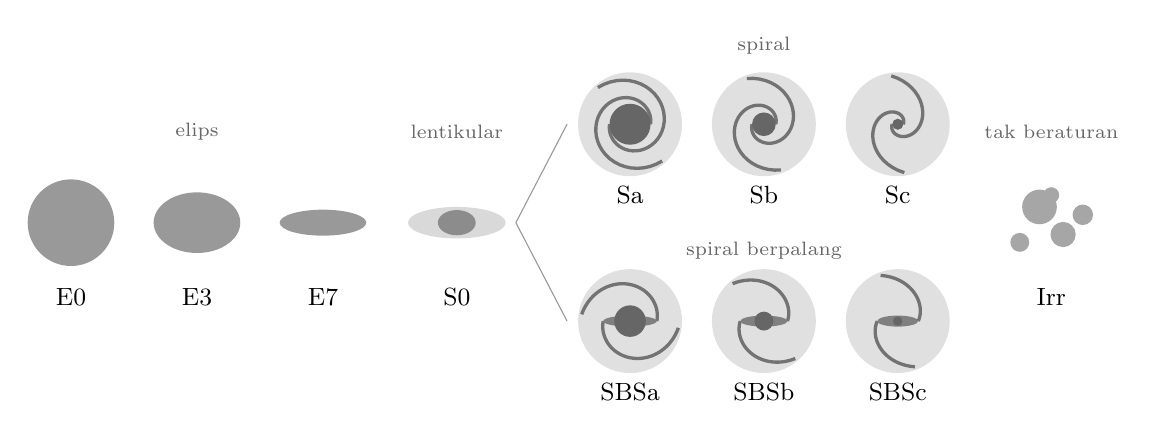
\begin{tikzpicture}[font=\small]
\def\spiralgal#1#2#3#4#5{% x, y, bulge radius, winding rate, bar half-length
  \begin{scope}[shift={(#1,#2)}]
    \fill[black!12] (0,0) circle (0.66);
    \pgfmathsetmacro{\rs}{max(#3,#5)}
    \pgfmathsetmacro{\th}{ln(0.62/\rs)/#4}
    \foreach \a in {0,180}
      \draw[line width=1.2pt, black!55, rotate=\a]
        plot[domain=0:\th, samples=40] ({\rs*exp(#4*\x)*cos(\x r)}, {\rs*exp(#4*\x)*sin(\x r)});
    \ifdim #5pt>0pt \fill[black!50] (0,0) ellipse (#5 and 0.07); \fi
    \fill[black!60] (0,0) circle (#3);
  \end{scope}}
\fill[black!40] (0,0) circle (0.55);
\fill[black!40] (1.6,0) ellipse (0.55 and 0.385);
\fill[black!40] (3.2,0) ellipse (0.55 and 0.165);
\fill[black!15] (4.9,0) ellipse (0.62 and 0.20);
\fill[black!45] (4.9,0) ellipse (0.24 and 0.16);
\draw[black!40] (5.65,0) -- (6.3,1.25);
\draw[black!40] (5.65,0) -- (6.3,-1.25);
\spiralgal{7.1}{1.25}{0.26}{0.16}{0}
\spiralgal{8.8}{1.25}{0.15}{0.28}{0}
\spiralgal{10.5}{1.25}{0.07}{0.45}{0}
\spiralgal{7.1}{-1.25}{0.20}{0.20}{0.34}
\spiralgal{8.8}{-1.25}{0.12}{0.32}{0.30}
\spiralgal{10.5}{-1.25}{0.06}{0.45}{0.26}
\foreach \p/\r in {(12.3,0.2)/0.22,(12.6,-0.15)/0.16,(12.05,-0.25)/0.12,(12.45,0.35)/0.1,(12.85,0.1)/0.13}
  \fill[black!35] \p circle (\r);
\foreach \x/\t in {0/E0,1.6/E3,3.2/E7,4.9/S0}
  \node at (\x,-0.95) {\t};
\foreach \x/\t in {7.1/Sa,8.8/Sb,10.5/Sc}
  { \node at (\x,0.35) {\t}; \node at (\x,-2.15) {SB\t}; }
\node at (12.45,-0.95) {Irr};
\node[font=\scriptsize, black!60] at (1.6,1.15) {elips};
\node[font=\scriptsize, black!60] at (4.9,1.15) {lentikular};
\node[font=\scriptsize, black!60] at (8.8,2.25) {spiral};
\node[font=\scriptsize, black!60] at (8.8,-0.35) {spiral berpalang};
\node[font=\scriptsize, black!60] at (12.45,1.15) {tak beraturan};
\end{tikzpicture}
\par\smallskip{\small \omterm{def:b3:milky-way-galaxies:types}{Deret Hubble} digambarkan seperti garpu penala,
secara skematis. \omterm{def:b3:milky-way-galaxies:types}{Galaksi elips} diberi label menurut kepipihan tampaknya;
garpu itu bercabang di \omterm{def:b3:milky-way-galaxies:types}{galaksi lentikular} menjadi spiral biasa dan spiral berpalang,
diurutkan dari tonjolan besar dan lengan terpilin rapat (a) hingga tonjolan kecil dan
lengan terbuka (c); \omterm{def:b3:milky-way-galaxies:types}{galaksi tak beraturan} menutup deret ini.}\label{fig:b3:milky-way-galaxies:fork}
\end{omfigure}
% ledger: buta11:hubble

Kelas-kelas ini menggambarkan bentuk yang terlihat di langit, dan satu label menyembunyikan
rentang: sebuah \omterm{def:b3:milky-way-galaxies:types}{galaksi elips} yang dilihat sepanjang sumbu terpendeknya tampak bulat, berapa pun
kepipihan sebenarnya, dan batas antara kelas-kelas yang bertetangga adalah
soal pertimbangan. Dalam katalog galaksi-galaksi di sekitar kita,
Bima Sakti tercatat sebagai S(B)bc, spiral di antara Sb dan Sc dengan batang; tetangga besarnya,
Andromeda (M31) adalah Sb, galaksi Segitiga (M33) adalah Sc, dan
Awan Magellan Besar dan Kecil adalah \omterm{def:b3:milky-way-galaxies:types}{galaksi tak beraturan}.
% ledger: buta11:hubble, mcconn12:local-group

\begin{omfigure}
\centering
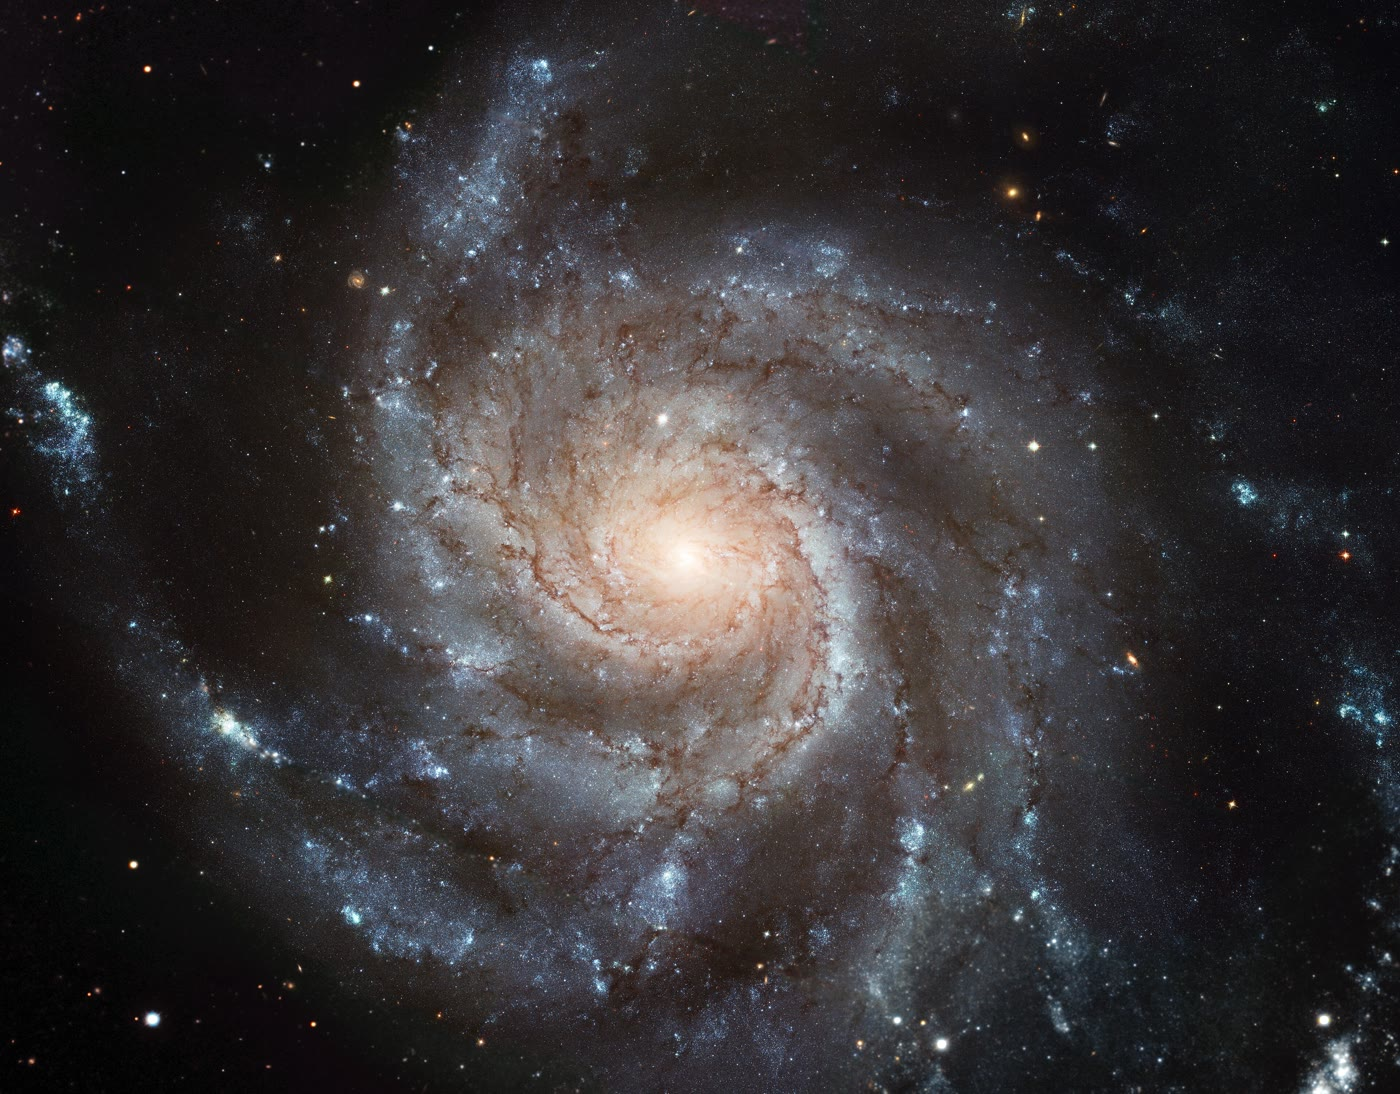
\includegraphics[width=0.66\linewidth]{images/book5/b3-m101.jpg}
\par\smallskip{\small \omterm{def:b3:milky-way-galaxies:types}{Galaksi spiral} M101 yang dilihat dari depan oleh Teleskop
Luar Angkasa Hubble, sebuah mosaik dari 51 eksposur, dipotong di tepinya: tonjolan
kecil, terang, kekuningan; lengan terbuka, lebih biru dan bergumpal dengan gugus
bintang muda; jalur debu cokelat di sepanjang lengan. Gambar ESA dan NASA
(Hubble, heic0602), CC BY~4.0.}\label{fig:b3:milky-way-galaxies:m101}
\end{omfigure}
% ledger: photo:b3-m101

Mengapa lengan spiral tidak terpilin rapat? Pada cakram yang \omterm{def:b3:milky-way-galaxies:rotation-curve}{kurva rotasinya} datar,
sebuah bintang pada setengah jarak dari pusat beredar dalam setengah waktu.
Sebuah spiral bintang akan makin rapat terpilin pada setiap putarannya, dan setelah
beberapa putaran cakram itu menjadi gulungan rapat (\cref{exo:b3:milky-way-galaxies:11}).

\begin{definition}[Teori gelombang massa jenis]\label{def:b3:milky-way-galaxies:density-wave}
Yang disebut \emph{teori gelombang massa jenis}\index{teori gelombang massa jenis} menjelaskan lengan spiral
sebagai gelombang massa jenis yang lebih tinggi di dalam cakram, sebuah pola spiral yang berputar
kaku dengan kelajuan sudutnya sendiri, yaitu kelajuan pola, sementara bintang dan
gas bergerak melewatinya, melambat ketika memasuki lengan yang padat dan
kembali bergerak cepat ketika keluar, seperti mobil yang melintasi kemacetan lalu lintas.
\end{definition}

Teori yang diajukan pada 1964 ini membebaskan lengan dari masalah pemilinan.
Gas yang memasuki lengan dipadatkan, dan bintang terbentuk di sana: lengan
ditandai oleh bintang muda dan gas yang berpendar, sementara bintang tua tersebar
jauh lebih merata. Apakah lengan berupa gelombang yang berumur panjang masih diperdebatkan;
simulasi komputer pada cakram lebih sering menumbuhkan lengan yang sementara,
larut dan terbentuk kembali, dan sebuah galaksi yang melintas atau sebuah batang dapat memicu
spiral dua lengan.
% ledger: dobbs14:density-wave

\begin{definition}[Lubang hitam supermasif]\label{def:b3:milky-way-galaxies:smbh}
Yang disebut \emph{lubang hitam supermasif}\index{lubang hitam supermasif} adalah lubang hitam
dengan massa satu juta massa Matahari atau lebih di pusat sebuah galaksi.
\end{definition}

Di pusat Galaksi, sumber radio kompak Sagittarius~A*
(Sgr~A*) berada di antara bintang-bintang pada orbit rapat dan cepat. Orbit-orbitnya memerlukan
massa pusat sekitar empat juta matahari, $\num[separate-uncertainty=true]{4.2 \pm 0.2 e6}$
massa Matahari menurut satu tinjauan atas pengukuran. Sgr~A* hampir tidak bergerak
relatif terhadap galaksi-galaksi jauh: setelah orbit Matahari dikeluarkan, gerak
sisanya paling besar beberapa kilometer per detik, jadi ia menampung
setidaknya seperempat massa itu. Ukurannya sebanding dengan jari-jari Schwarzschild-nya,
dan massa jenisnya, di atas \num{4e23} massa Matahari per
parsek kubik, sangat dekat dengan yang diharapkan bagi lubang hitam: bukti
bahwa Sgr~A* adalah lubang hitam sangat meyakinkan.
% ledger: reid20:sgra, bhg16:structure, gravity19:r0

\begin{definition}[Grup Lokal; gugus galaksi]\label{def:b3:milky-way-galaxies:groups}
Yang disebut \emph{Grup Lokal}\index{Grup Lokal} adalah kelompok galaksi terikat gravitasi
yang didominasi Bima Sakti dan Andromeda, masing-masing dengan
galaksi satelitnya. Yang disebut \emph{gugus galaksi}\index{gugus galaksi} adalah
salah satu sistem terikat gravitasi terbesar: banyak galaksi yang tertahan,
bersama gas panas yang memancarkan sinar-X, di dalam sumur gravitasi bersama yang
sebagian besar berupa materi gelap.
\end{definition}

Lebih dari seratus galaksi berada dalam jarak \qty{3}{Mpc} dari Matahari, sebagian besar
berupa galaksi kerdil. Large Magellanic Cloud berada pada sekitar \qty{50}{kpc}, Andromeda pada
\qty{783}{kpc} dan mendekati kita dengan kecepatan \qty{300}{km.s^{-1}}, serta anggota yang terikat
dari grup berada dalam sekitar \qty{1.06}{Mpc} dari pusat
massa, di antara Galaksi dan Andromeda, tempat mereka menyimpang dari
ekspansi Alam Semesta. Massanya, dari gerak dua galaksi besar
yang saling mendekat, berorde \num{5e12} massa Matahari. Dalam
\omterm{def:b3:milky-way-galaxies:groups}{gugus galaksi} masif, gas panas pada sekitar \qty{e8}{K} menampung sekitar sepuluh
kali massa bintangnya; galaksi dan gas bersama terlalu ringan untuk
kedalaman sumur gravitasi, dan sebagian besar massa gugus itu,
berorde \num{e15} massa Matahari, adalah materi gelap.
% ledger: mcconn12:local-group, kravtsov12:clusters

\section{Tangga jarak}\label{sec:b3:milky-way-galaxies:ladder}

Paralaks memberikan jarak hanya dengan geometri, tetapi paralaks mengecil
seiring bertambahnya jarak. Katalog terbaik untuk itu mengukur paralaks dengan
ketidakpastian 0.02 sampai \qty{0.03}{mas} untuk bintang yang lebih terang daripada
magnitudo~15, sehingga jarak dengan ketidakpastian \qty{10}{\percent} sampai sekitar
\qty{4}{kpc}; Large Magellanic Cloud, pada \qty{50}{kpc}, memiliki sebuah
paralaks sebesar \qty{0.02}{mas}. Di luar itu, jarak bertumpu pada objek
yang luminositasnya diketahui.
% ledger: gaia:dr3, freedman19:trgb

\begin{definition}[Lilin standar; tangga jarak]\label{def:b3:milky-way-galaxies:ladder}
Yang disebut \emph{lilin standar}\index{lilin standar} adalah kelas objek
yang magnitudo mutlaknya diketahui, atau dapat diturunkan dari suatu sifat
yang diukur secara independen dari jarak, sehingga magnitudo semunya memberikan
modulus jaraknya. Yang disebut \emph{tangga jarak}\index{tangga jarak} adalah
rangkaian metode, masing-masing dikalibrasi pada objek yang cukup dekat untuk
juga diukur dengan metode sebelumnya, yang membawa jarak dari
paralaks hingga ke Alam Semesta yang sedang mengembang.
\end{definition}

\begin{definition}[Variabel Cepheid; hukum Leavitt]\label{def:b3:milky-way-galaxies:cepheid}
Yang disebut \emph{variabel Cepheid}\index{variabel Cepheid} adalah bintang muda yang terang dan berdenyut,
yang kecerlangannya berubah dengan periode yang benar-benar teratur,
dari sekitar satu hari hingga beberapa minggu. Yang disebut \emph{hukum Leavitt}\index{hukum Leavitt},
atau relasi periode--luminositas, adalah relasi linear antara rata-rata magnitudo mutlak
sebuah Cepheid dan logaritma periodenya, dengan periode
yang lebih panjang untuk bintang yang lebih terang.
\end{definition}

Relasi ini ditemukan di Small Magellanic Cloud, yang bintang-bintangnya
semuanya berada pada jarak yang hampir sama, pada 1908. Debu di galaksi yang
menampung sebuah Cepheid meredupkan dan memerahkannya; tetapi peredupannya lebih besar
pada cahaya tampak daripada pada inframerah dekat, dengan rasio tetap untuk jenis
debu tertentu, dan kombinasi $W_I = I - 1.55\,(V - I)$ dari magnitudo pada
pita I dan V, indeks Wesenheit, dipilih agar peredupannya
saling meniadakan. Gambar di bawah ini menunjukkannya untuk 2315 Cepheid di
Large Magellanic Cloud: \omterm{def:b3:milky-way-galaxies:cepheid}{hukum Leavitt} berupa garis rapat, dengan sebaran
\qty{0.078}{mag}, yaitu \qty{3.6}{\percent} dalam jarak untuk satu
bintang.
% ledger: sos15:leavitt, data:b5-ogle-lmc-cep

\begin{omfigure}
\centering
\begin{tikzpicture}
\begin{axis}[width=0.80\linewidth, height=0.52\linewidth,
  xmin=-0.05, xmax=1.6, ymin=10, ymax=16.6, y dir=reverse,
  xlabel={$\log_{10}(P/\mathrm{d})$}, ylabel={indeks Wesenheit $W_I$ (mag)},
  tick label style={font=\scriptsize}, label style={font=\small},
  legend style={font=\scriptsize, at={(0.5,-0.17)}, anchor=north, legend columns=3, draw=none, cells={anchor=west}, /tikz/every even column/.append style={column sep=1em}},
  legend image post style={scale=2.2}]
\addplot[only marks, mark=*, mark size=0.45pt, omDef, opacity=0.6] table[x=logp, y=w] {figdata/out/bachelor-3-distance_ladder-pl.dat};
\addlegendentry{Cepheid}
\addplot[only marks, mark=x, mark size=1.6pt, red!70!black] table[x=logp, y=w] {figdata/out/bachelor-3-distance_ladder-clipped.dat};
\addlegendentry{disisihkan ($>3\sigma$)}
\addplot[thick, black] table[x=logp, y=w_fit] {figdata/out/bachelor-3-distance_ladder-fit.dat};
\addlegendentry{garis suai}
\node[font=\scriptsize, anchor=south west, fill=white, inner sep=1pt] at (axis cs:0.55,11.0) {$W_I = -3.315\log_{10}P + 15.889$};
\end{axis}
\end{tikzpicture}
\par\smallskip{\small \omterm{def:b3:milky-way-galaxies:cepheid}{Hukum Leavitt} di Large Magellanic Cloud:
indeks Wesenheit dari 2315 Cepheid yang berdenyut pada mode fundamentalnya
terhadap logaritma periodenya (survei OGLE, Soszy\'nski dan
dkk., 2015, melalui CDS). Bintang yang lebih terang berada lebih tinggi.
Garis lurus yang dicocokkan dengan kuadrat terkecil, setelah menyisihkan 92 bintang yang lebih dari tiga
simpangan baku darinya, mereproduksi relasi yang dipublikasikan
($-3.314$, $15.888$). Dengan modulus jarak awan itu, 18.477, garis
memberikan magnitudo mutlak Wesenheit dari setiap Cepheid berdasarkan periodenya.}\label{fig:b3:milky-way-galaxies:leavitt}
\end{omfigure}
% ledger: data:b5-ogle-lmc-cep, sos15:leavitt, freedman19:trgb

\begin{definition}[Ujung cabang raksasa merah]\label{def:b3:milky-way-galaxies:trgb}
Yang disebut \emph{ujung cabang raksasa merah}\index{ujung cabang raksasa merah}
(TRGB) adalah batas atas yang tajam bagi luminositas raksasa merah dari
\omterm{def:b3:milky-way-galaxies:populations}{populasi bintang} tua yang ditentukan oleh penyalaan helium di dalam inti mereka,
kilatan helium; di pita I, magnitudo mutlaknya hampir sama di
setiap populasi tua, $M_I \approx -4.05$ pada warna
$V - I = 1.6$, hanya bergantung lemah pada komposisi kimia.
\end{definition}

Ujung ini diukur di halo galaksi yang renggang, tempat terdapat sedikit
debu dan sedikit kerapatan bintang; ia memakai bintang halo tua tempat Cepheid memakai
bintang cakram muda, dan kedua metode itu tidak berbagi fisika. Cepheid dan
TRGB mencapai beberapa puluh megaparsek, ke galaksi tempat sebuah \omterm{def:b3:milky-way-galaxies:ladder}{lilin standar} yang langka dan jauh
lebih terang telah meledak: supernova Tipe~Ia, yaitu ledakan
termonuklir sebuah katai putih yang sudah dibahas di buku fisika,
yang magnitudo mutlak puncaknya, setelah dikoreksi untuk
bentuk kurva cahayanya dan warnanya, adalah
$M_B = \qty[separate-uncertainty=true]{-19.253 \pm 0.027}{mag}$. Supernova seperti
itu teramati sampai ratusan megaparsek.
% ledger: freedman19:trgb, riess22:h0

\begin{definition}[Relasi Tully--Fisher]\label{def:b3:milky-way-galaxies:tully-fisher}
Yang disebut \emph{relasi Tully--Fisher}\index{relasi Tully--Fisher} adalah
korelasi antara luminositas, atau lebih tepatnya massa bintang dan gas,
dari \omterm{def:b3:milky-way-galaxies:types}{galaksi spiral} dan kelajuan \omterm{def:b3:milky-way-galaxies:rotation-curve}{kurva rotasinya} yang datar; dalam bentuk
baryonik, $M_\mathrm{b} = A\,V^4$, berlaku dari sekitar 30 sampai
\qty{300}{km.s^{-1}}.
\end{definition}

Spektrum 21-cm sebuah galaksi memberikan kelajuan rotasi maksimumnya, relasi
memberikan luminositasnya tanpa bergantung pada jaraknya, dan fluksnya
kemudian memberikan jarak: sebuah anak tangga bagi \omterm{def:b3:milky-way-galaxies:types}{galaksi spiral} yang terlalu jauh untuk
bintang tunggal. Bima Sakti, dengan luminositas dan rotasinya, jatuh pada relasi itu.
% ledger: mcgaugh00:btf, nrao:hi-line, bhg16:structure

\begin{omfigure}
\centering
\pgfplotstableread{figdata/out/bachelor-3-distance_ladder-ladder.dat}\laddertab
\pgfplotstableread{figdata/out/bachelor-3-distance_ladder-anchors.dat}\anchortab
\pgfplotstablegetelem{0}{d_hi}\of{\laddertab}\let\plxhi\pgfplotsretval
\pgfplotstablegetelem{1}{d_lo}\of{\laddertab}\let\cephlo\pgfplotsretval
\pgfplotstablegetelem{1}{d_hi}\of{\laddertab}\let\cephhi\pgfplotsretval
\pgfplotstablegetelem{3}{d_lo}\of{\laddertab}\let\snlo\pgfplotsretval
\pgfplotstablegetelem{3}{d_hi}\of{\laddertab}\let\snhi\pgfplotsretval
\pgfplotstablegetelem{1}{d}\of{\anchortab}\let\mthirtyone\pgfplotsretval
\pgfplotstablegetelem{2}{d}\of{\anchortab}\let\nfourtwo\pgfplotsretval
\begin{tikzpicture}
\begin{axis}[width=0.92\linewidth, height=0.42\linewidth,
  xmode=log, xmin=1e-3, xmax=2e6, ymin=0.4, ymax=4.9,
  ytick={1,2,3,4}, yticklabels={paralaks, Cepheid, TRGB, SNe~Ia},
  xtick={1e-3,1e-2,1e-1,1,10,100,1e3,1e4,1e5,1e6},
  xticklabels={1\,pc,,,1\,kpc,,,1\,Mpc,,,1\,Gpc},
  xlabel={jarak}, tick label style={font=\scriptsize}, label style={font=\small},
  y tick label style={font=\small}, axis y line*=left, axis x line*=bottom]
\draw[line width=7pt, omDef!70] (axis cs:1e-3,1) -- (axis cs:\plxhi,1);
\draw[line width=7pt, omMeth!70] (axis cs:\cephlo,2) -- (axis cs:\cephhi,2);
\draw[line width=7pt, omProp!70] (axis cs:\cephlo,3) -- (axis cs:\cephhi,3);
\draw[line width=7pt, red!60] (axis cs:\snlo,4) -- (axis cs:\snhi,4);
\draw[densely dotted, thick] (axis cs:\cephlo,0.4) -- (axis cs:\cephlo,4.55) node[anchor=south, font=\scriptsize] {LMC};
\draw[densely dotted, thick] (axis cs:\mthirtyone,0.4) -- (axis cs:\mthirtyone,4.55) node[anchor=south, font=\scriptsize] {M31};
\draw[densely dotted, thick] (axis cs:\nfourtwo,0.4) -- (axis cs:\nfourtwo,4.55) node[anchor=south, font=\scriptsize] {NGC~4258};
\draw[->, thick, black!60] (axis cs:\plxhi,1.25) to[out=30, in=200] (axis cs:\cephlo,1.75);
\draw[->, thick, black!60] (axis cs:\cephhi,2.25) to[out=40, in=220] (axis cs:\snlo,3.75);
\end{axis}
\end{tikzpicture}
\par\smallskip{\small Anak tangga dari \omterm{def:b3:milky-way-galaxies:ladder}{tangga jarak}, dengan
jarak tempat masing-masing dipakai di sini: paralaks dari katalog terbaik,
hingga \qty{10}{\percent} sampai \qty{4}{kpc}; Cepheid dan TRGB mulai dari
Large Magellanic Cloud sampai ke inang supernova Tipe~Ia terdekat,
\qty{45}{Mpc}; supernova dari pemuaian yang mulus, pada pergeseran merah 0.023
sampai 0.15 (\qtyrange{96}{616}{Mpc} untuk $H_0 = 73$). Garis putus-putus: dua jangkar
skala Cepheid dengan jarak geometris (binari gerhana di
LMC, maser air yang mengorbit lubang hitam NGC~4258), dan M31, \omterm{def:b3:milky-way-galaxies:types}{galaksi
spiral} besar terdekat. Panah: setiap anak tangga dikalibrasi pada objek yang
juga diukur oleh anak tangga di bawahnya, yaitu Cepheid Bima Sakti dengan paralaksnya,
supernova galaksi terdekat oleh Cepheid dan TRGB dari
inangnya.}\label{fig:b3:milky-way-galaxies:ladder-rungs}
\end{omfigure}
% ledger: gaia:dr3, riess22:h0, freedman19:trgb, mcconn12:local-group

Di puncak tangga itu, supernova mengukur pemuaian
Alam Semesta. Hukum Hubble, yang sudah dibahas di buku fisika, membuat laju
resesi $cz$ galaksi yang jauh sebanding dengan jaraknya $d$,
$cz = H_0 d$ untuk pergeseran merah $z$ yang kecil; konstanta Hubble $H_0$ adalah
gradien, dan supernova, dengan jarak mereka dari tangga, memberikannya.

\begin{definition}[Ketegangan Hubble]\label{def:b3:milky-way-galaxies:tension}
Yang disebut \emph{ketegangan Hubble}\index{ketegangan Hubble} ialah ketidaksesuaian
antara nilai konstanta Hubble yang diukur secara lokal dengan
\omterm{def:b3:milky-way-galaxies:ladder}{tangga jarak} dan nilai yang diturunkan dari latar gelombang mikro
kosmik dengan model kosmologi standar.
\end{definition}

\begin{dated}{2022}
Cepheid di inang 42 supernova Tipe~Ia, dijangkarkan pada
paralaks Gaia, maser NGC~4258, dan binari gerhana dari
Large Magellanic Cloud, memberikan
$H_0 = \qty[separate-uncertainty=true]{73.04 \pm 1.04}{km.s^{-1}.Mpc^{-1}}$.
\omterm{def:b3:milky-way-galaxies:trgb}{Ujung cabang raksasa merah}, yang dikalibrasi pada sekitar seratus supernova,
memberikan pada 2019 $H_0 = 69.8 \pm 0.8 \pm \qty{1.7}{km.s^{-1}.Mpc^{-1}}$
(statistik dan sistematik). Peta satelit Planck tentang latar gelombang mikro
kosmik, dibaca dengan model kosmologi standar, menyiratkan
$H_0 = \qty[separate-uncertainty=true]{67.4 \pm 0.5}{km.s^{-1}.Mpc^{-1}}$.
Nilai Cepheid dan nilai latar berbeda lima
simpangan baku; nilai TRGB berada di antara keduanya. Sumber
ketidaksesuaian ini belum diketahui: kesalahan yang belum ditemukan pada salah satu
tangga, atau fisika yang hilang dari model.
\end{dated}
% ledger: riess22:h0, freedman19:trgb, planck18:h0

\begin{inthelab}[Satelit astrometrik dan katalognya]
Satelit Gaia memindai langit sepanjang pola yang telah ditentukan, sehingga setiap
bintang diukur berulang kali selama misinya. Di Bumi, unit-unit koordinasi
dari konsorsium pengolahan data mengubah pengukuran-pengukuran ini
menjadi posisi, paralaks, dan gerak diri untuk setiap
lebih dari satu miliar sumber. Dari gerak kecil bintang di langit,
paralaks adalah bagian yang berulang setiap tahun, dan gerak diri
adalah bagian yang terakumulasi. Setiap katalog dirilis bersama makalah yang
menjelaskan pengolahan dan validasinya, dan setiap jarak dalam
gambar pada bagian ini yang bertumpu pada paralaks juga bertumpu pada
katalog semacam itu.
\end{inthelab}

\begin{dated}{2022}
Katalog Gaia ketiga, dirilis pada 13 Juni 2022 dari 34 bulan
pengamatan, memuat posisi, paralaks, dan gerak diri untuk sekitar
1.46~miliar sumber, dengan magnitudo~3 hingga~21, dan kecepatan radial rata-rata
untuk 33~juta bintang. Ketidakpastian paralaksnya sebesar 0.02 hingga
\qty{0.03}{mas} untuk bintang yang lebih terang dari magnitudo~15, \qty{0.07}{mas} pada
magnitudo~17, dan \qty{0.5}{mas} pada magnitudo~20.
\end{dated}
% ledger: gaia:dr3

\section{Latihan}

\begin{exercise}[$\star$]\label{exo:b3:milky-way-galaxies:1}
Tahun Galaksi Matahari. (a)~Dengan $R_0 = \qty{8.178}{kpc}$ dan
$V_0 = \qty{229}{km.s^{-1}}$, hitung periode orbit Matahari mengelilingi
pusat Galaksi, dalam juta tahun. (b)~Berapa kali Matahari
telah mengelilingi pusat sejak Tata Surya terbentuk, \qty{4.54}{Ga} yang lalu?
\end{exercise}

\begin{exercise}[$\star$]\label{exo:b3:milky-way-galaxies:2}
Gerak reaksi Sgr~A*. (a)~Gerak diri sebesar \qty{1}{mas} per tahun
pada \qty{1}{kpc} setara dengan kecepatan transversal \qty{1}{au} per tahun: nyatakan dalam
kilometer per detik. (b)~Sgr~A*, diasumsikan diam di pusat Galaksi
pada \qty{8.178}{kpc}, bergeser sepanjang bidang Galaksi sebesar \qty{6.411}{mas}
per tahun. Hitung kecepatan Matahari mengelilingi pusat dan bandingkan dengan
nilai acuan, \qty[separate-uncertainty=true]{248 \pm 3}{km.s^{-1}}. (c)~Kurangi gerak
peculiar Matahari searah rotasi, \qty{11}{km.s^{-1}}, lalu
bandingkan dengan $V_0$ dari \omterm{def:b3:milky-way-galaxies:rotation-curve}{kurva rotasi}.
\end{exercise}

\begin{exercise}[$\star$]\label{exo:b3:milky-way-galaxies:3}
Mengklasifikasikan \omterm{def:b3:milky-way-galaxies:types}{galaksi elips}. (a)~Isofot \omterm{def:b3:milky-way-galaxies:types}{galaksi elips} memiliki
rasio sumbu 0.6: tentukan kelasnya. (b)~Berapa rasio sumbu yang dimiliki E7?
(c)~Mengapa galaksi E0 bisa berupa sistem yang tergepengkan?
\end{exercise}

\begin{exercise}[$\star$]\label{exo:b3:milky-way-galaxies:4}
Titik acuan. Hitung jarak Awan Magellan Besar
($\mu = 18.477$), Andromeda ($\mu = 24.47$), dan NGC~4258
($\mu = 29.398$). Berapa paralaks yang dimiliki sebuah bintang di Awan itu, dan mengapa
jarak Awan itu tidak dapat diukur dengan paralaks?
\end{exercise}

\begin{exercise}[$\star\star$]\label{exo:b3:milky-way-galaxies:5}
Dari \omterm{def:b3:milky-way-galaxies:rotation-curve}{konstanta Oort} $A = \qty{15.3}{km.s^{-1}.kpc^{-1}}$ dan
$B = \qty{-11.9}{km.s^{-1}.kpc^{-1}}$: (a)~hitung kecepatan sudut
\omterm{def:b3:milky-way-galaxies:lsr}{standar diam lokal} dan, dengan $R_0 = \qty{8.178}{kpc}$, kecepatan melingkar $V_0$;
(b)~hitung kemiringan \omterm{def:b3:milky-way-galaxies:rotation-curve}{kurva rotasi} di posisi Matahari. (c)~Bandingkan
dengan \omterm{def:b3:milky-way-galaxies:rotation-curve}{kurva rotasi} raksasa merah ($V_0 = \qty{229.0}{km.s^{-1}}$,
kemiringan \qty{-1.7}{km.s^{-1}} per kiloparsek) dan sarankan mengapa keduanya
berbeda, mengingat pengukuran yang sama menemukan $C$ dan $K$ tidak nol.
\end{exercise}

\begin{exercise}[$\star\star$]\label{exo:b3:milky-way-galaxies:6}
\omterm{def:b3:milky-way-galaxies:rotation-curve}{Kurva rotasi} datar dan massa jenis lokal. (a)~Untuk galaksi berbentuk bola
dengan \omterm{def:b3:milky-way-galaxies:rotation-curve}{kurva rotasi} datar pada \qty{229}{km.s^{-1}}, hitung massa jenis di
\qty{8.178}{kpc}, dalam massa Matahari per parsek kubik
($G = \qty{4.301e-6}{kpc.(km.s^{-1})^2}$ per massa Matahari). (b)~Tunjukkan bahwa
satu massa Matahari per parsek kubik setara dengan \qty{37.96}{GeV.cm^{-3}}, dan nyatakan
massa jenis materi gelap lokal, \qty{0.30}{GeV.cm^{-3}}, dalam massa Matahari
per parsek kubik. (c)~Mengapa massa jenis pada (a) lebih besar?
\end{exercise}

\begin{exercise}[$\star\star$]\label{exo:b3:milky-way-galaxies:7}
Jarak \omterm{def:b3:milky-way-galaxies:cepheid}{variabel Cepheid}. Dalam \omterm{def:b3:milky-way-galaxies:types}{galaksi spiral} rekaan, sebuah \omterm{def:b3:milky-way-galaxies:cepheid}{variabel Cepheid} dengan periode
\qty{30}{d} memiliki indeks Wesenheit rata-rata $W_I = \qty{25.00}{mag}$.
(a)~Dengan \omterm{def:b3:milky-way-galaxies:cepheid}{hukum Leavitt} untuk Awan Magellan Besar,
$W_I = -3.314\log_{10}P + 15.888$, dan modulus jarak Awan itu
18.477, hitung magnitudo mutlak Wesenheit Cepheid tersebut. (b)~Hitung
jarak galaksi itu. (c)~Sebaran hukum ini sebesar \qty{0.077}{mag}: berapa
kesalahan jarak relatif dari satu Cepheid, dan dari lima puluh?
\end{exercise}

\begin{exercise}[$\star\star$]\label{exo:b3:milky-way-galaxies:8}
Jarak TRGB. Di halo sebuah galaksi rekaan, \omterm{def:b3:milky-way-galaxies:trgb}{ujung cabang raksasa
merah} ditemukan pada $I = \qty{26.00}{mag}$; debu di sepanjang garis pandang
meredupkan pita I sebesar \qty{0.05}{mag}. Dengan $M_I = -4.05$, hitung
modulus jarak dan jaraknya. Apa arti ketidakpastian
\qty{0.04}{mag} pada ujung itu dalam hal jarak?
\end{exercise}

\begin{exercise}[$\star\star$]\label{exo:b3:milky-way-galaxies:9}
Konstanta Hubble dari supernova. Untuk supernova dengan ekspansi
halus, $\log_{10}(cz) - 0.2\,m_B = a_B$, perpotongan diagram Hubble
supernova, dan modulus jarak diberikan oleh
$m_B - M_B = 5\log_{10}(d/\mathrm{Mpc}) + 25$. (a)~Tunjukkan bahwa
$\log_{10}H_0 = 0.2\,M_B + a_B + 5$ ($H_0$ dalam kilometer per detik per
megaparsek). (b)~Dengan $M_B = -19.253$ dan $a_B = 0.714158$, hitung $H_0$.
(c)~Berapa $M_B$ yang memberi $H_0 = \qty{67.4}{km.s^{-1}.Mpc^{-1}}$? Dengan
berapa magnitudo, dan dengan pecahan jarak berapa, kedua
kalibrasi itu berbeda?
\end{exercise}

\begin{exercise}[$\star\star\star$]\label{exo:b3:milky-way-galaxies:10}
Asal hukum Tully--Fisher. (a)~Galaksi cakram bermassa $M$
dan jari-jari $R$ berputar dengan kecepatan $V$: tunjukkan bahwa $M \approx RV^2/G$. (b)~Jika semua
\omterm{def:b3:milky-way-galaxies:types}{galaksi spiral} memiliki massa jenis permukaan rata-rata $\Sigma = M/(\pi R^2)$ yang sama,
tunjukkan bahwa $M \propto V^4$. (c)~Dua galaksi rekaan pada relasi barionik yang sama
berputar pada 100 dan \qty{229}{km.s^{-1}}: berapa rasio
massanya? (d)~Dua galaksi berputar dengan kecepatan sama dan memiliki luminositas yang sama;
satu di antaranya memberikan fluks empat kali lipat dari yang lain. Bandingkan
jaraknya.
\end{exercise}

\begin{exercise}[$\star\star\star$]\label{exo:b3:milky-way-galaxies:11}
Masalah pelilitan. Sebuah cakram berputar dengan kurva datar pada
\qty{229}{km.s^{-1}}. (a)~Ubah kelajuan ini menjadi kiloparsek per miliar
tahun. (b)~Sebuah lengan bintang lurus pada waktu nol membentang dari 4 hingga
\qty{12}{kpc}. Hitung periode orbit di kedua ujungnya. (c)~Setelah
\qty{1}{Ga}, sebesar sudut berapa ujung dalamnya telah mendahului ujung
luarnya? Berapa putaran spiral itu, dan bagaimana tampilan lengannya?
(d)~Bagaimana gelombang massa jenis menghindari hal ini?
\end{exercise}

\begin{exercise}[$\star\star\star$]\label{exo:b3:milky-way-galaxies:12}
Lubang hitam di pusat. Anggap massa pusat sebesar
\num{4.2e6} massa Matahari dan $R_0 = \qty{8178}{pc}$. (a)~Bintang S2
mengorbit di sekitarnya dalam \num{16}~tahun: hitung sumbu semi-mayor orbitnya dalam
satuan astronomi (hukum Kepler ketiga dalam satuan Matahari, $a^3 = MP^2$ dengan
$a$ dalam au, $P$ dalam tahun, dan $M$ dalam massa Matahari) serta ukuran sudutnya yang terlihat
dari Bumi. (b)~Hitung jari-jari Schwarzschild lubang hitam dalam
meter dan dalam satuan astronomi, serta sudut yang dibentuk diameternya
dari Bumi, dalam mikrodetik busur. (c)~Hitung massa jenis rata-rata dari
massa di dalam jari-jari Schwarzschild-nya, dalam massa Matahari per parsek
kubik, dan bandingkan dengan batas bawah yang ditetapkan oleh gerak Sgr~A*,
\num{4e23} massa Matahari per parsek kubik.
\end{exercise}

\section{Soal: Menimbang Galaksi}

\begin{problem}[{Soal akhir pekan --- dari gerak bintang dan gas hingga
materi gelap dalam \qty{20}{kpc}}]
\label{pb:b3:milky-way-galaxies:1}
Ambil $R_0 = \qty{8.18}{kpc}$, $G = \qty{4.301e-6}{kpc.(km.s^{-1})^2}$ per
massa Matahari, dan \qty{4.74}{km.s^{-1}} untuk gerak diri sebesar
\qty{1}{mas} per tahun pada \qty{1}{kpc}. Semua kecepatan diukur relatif terhadap
LSR. Gunakan teorema Oort dan teorema titik-singgung yang ada di bab ini, serta
pendekatan bola $M = RV^2/G$ untuk massa dinamik.

\medskip\noindent\textbf{Bagian I --- Rotasi lokal.} Sebuah survei rekaan
terhadap bintang klamp merah, semuanya pada $d = \qty{1.00}{kpc}$ di bidang
Galaksi, memberikan kecepatan radial rata-rata \qty{+15.4}{km.s^{-1}} pada
$\ell = \ang{45}$ dan \qty{-15.2}{km.s^{-1}} pada $\ell = \ang{135}$, serta
gerak diri rata-rata pada arah bujur sebesar \qty{-5.91}{mas} per tahun pada
$\ell = \ang{90}$ dan \qty{+0.55}{mas} per tahun pada $\ell = \ang{0}$.
\begin{enumerate}
\item Apa yang diprediksi rumus Oort untuk kecepatan radial pada
  $\ell = \ang{45}$, \ang{90}, \ang{135} dan \ang{180}?
\item Hitung $A$ dari kedua kecepatan radial itu.
\item Hitung $B$ dari gerak diri pada $\ell = \ang{90}$.
\item Hitung kembali $B$ dari gerak diri pada $\ell = \ang{0}$, lalu
  bandingkan.
\item Hitung kecepatan sudut LSR dan kecepatan melingkar
  $V_0$.
\item Hitung kemiringan \omterm{def:b3:milky-way-galaxies:rotation-curve}{kurva rotasi} di Matahari. Apakah kurva itu naik,
  datar atau turun?
\item Hitung periode orbit Matahari dan jumlah putaran dalam
  \qty{4.54}{Ga}.
\end{enumerate}

\medskip\noindent\textbf{Bagian II --- Kurva rotasi bagian dalam.} Ambil
$V_0 = \qty{229}{km.s^{-1}}$. Kecepatan radial tertinggi dalam
profil 21-cm pada $\ell = \ang{40}$, \ang{50}, \ang{60} dan \ang{70} adalah
82.9, 55.6, 32.4 dan \qty{14.9}{km.s^{-1}}.
\begin{enumerate}[resume]
\item Mengapa metode titik-singgung memerlukan $\ang{0} < \ell < \ang{90}$
  (atau kuadran cerminnya), dan mengapa metode ini gagal di luar lingkaran Matahari?
\item Hitung jari-jari titik-singgung untuk setiap bujur.
\item Hitung $V(R)$ pada setiap titik-singgung.
\item Berapa besar, dalam kilohertz, garis gas pada titik-singgung di
  $\ell = \ang{40}$ bergeser dari frekuensi diamnya,
  \qty{1420.405751}{MHz}, dan ke arah mana?
\item Bandingkan dengan kurva raksasa merah, yang memberikan \qty{226.8}{km.s^{-1}}
  pada \qty{5.27}{kpc} dan \qty{229.6}{km.s^{-1}} pada \qty{7.22}{kpc}. Apakah
  kurva bagian dalam itu naik, datar atau turun?
\item Jika kecepatan di titik-singgung pada $\ell = \ang{40}$ adalah kecepatan
  titik massa di pusat yang membawa Matahari dengan $V_0$, berapakah nilainya?
  Apa yang dikatakan perbandingan ini tentang persebaran massa?
\end{enumerate}

\medskip\noindent\textbf{Bagian III --- Massa tampak.} Gunakan model massa
bab ini, dalam satuan massa Matahari dan kiloparsek: tonjolan Plummer
$M = \num{1.067e10}$, $b = 0.3$; cakram Miyamoto--Nagai tipis
$M = \num{3.944e10}$, $a = 5.3$, $b = 0.25$; satu \omterm{def:b3:milky-way-galaxies:structure}{cakram tebal} dengan
massa yang sama dengan $a = 2.6$, $b = 0.8$.
\begin{enumerate}[resume]
\item Hitung massa tampak total model dan bandingkan dengan nilai tinjauan
  massa bintang Galaksi, \qty[separate-uncertainty=true]{5 \pm 1 e10}{}
  massa Matahari.
\item Hitung kecepatan melingkar tonjolan saja pada \qty{20}{kpc}.
\item Hitung kecepatan melingkar cakram tipis dan \omterm{def:b3:milky-way-galaxies:structure}{cakram tebal} pada \qty{20}{kpc}.
\item Hitung kecepatan melingkar seluruh massa tampak pada
  \qty{20}{kpc}.
\item Hitung hal yang sama pada $R_0$, lalu bandingkan dengan $V_0$.
\item Jika seluruh massa tampak dipusatkan di tengah, berapakah kecepatannya
  pada \qty{20}{kpc}? Mengapa nilai model mendekatinya?
\end{enumerate}

\medskip\noindent\textbf{Bagian IV --- Materi gelap.} Raksasa merah
memberikan kecepatan melingkar \qty{200}{km.s^{-1}} pada \qty{20}{kpc}.
\begin{enumerate}[resume]
\item Hitung massa dinamik dalam \qty{20}{kpc}.
\item Hitung massa dinamik materi tampak dalam
  \qty{20}{kpc}.
\item Hitung massa materi gelap dalam \qty{20}{kpc}, dan tunjukkan bahwa
  pecahannya adalah $1 - (V_\mathrm{vis}/V)^2$.
\item Halo NFW yang dicocokkan dengan seluruh kurva memiliki
  $\rho_0 = \num{1.06e7}$ massa Matahari per kiloparsek kubik dan
  $R_s = \qty{14.8}{kpc}$. Hitung massanya dalam \qty{20}{kpc} serta
  pecahan gelap yang ditimbulkannya. Mengapa hasilnya berbeda dengan jawaban sebelumnya?
\item Hitung massa jenis halo itu pada $R_0$, dalam massa Matahari per
  parsek kubik dan dalam \unit{GeV.cm^{-3}} (satu massa Matahari per parsek kubik
  sama dengan \qty{37.96}{GeV.cm^{-3}}).
\item Berikan pecahan materi gelap dari massa dalam \qty{20}{kpc} yang
  diperoleh dari kecepatan terukur, dalam persen, hingga dua
  angka penting.
\end{enumerate}
\end{problem}
% ledger: gravity19:r0, eilers19:table1, pouliasis17:model1, eilers19:halo, bhg16:structure, nrao:hi-line, const:G, const:au, iau:parsec, usgs:age-earth
